\documentclass[11pt]{article}
\usepackage[latin1]{inputenc}
\usepackage{amsmath}
\usepackage{amsfonts}
\usepackage{amssymb}
\usepackage{graphicx}
\usepackage{setspace}
\usepackage[left=1.00in, right=1.00in, top=1.00in, bottom=1.00in]{geometry}
\usepackage[english]{babel}
%\setlength{\parindent}{0pt}
\newcommand{\forceindent}{\leavevmode{\parindent=1.5em\indent}} % em = roughly width of uppercase ``M", or just over a third of a cm

\usepackage{fancyhdr}

\pagestyle{fancy}
\fancyhf{}
\rhead{University of Houston $|$ Political Science}
\lhead{Learning \LaTeX: Week 4} %% BE SURE TO CHANGE THIS EACH WEEK
\rfoot{Page \thepage}

\graphicspath{/Users/bpwaggo/Dropbox/LaTeX Workshop Series/Week 4}
%\usepackage{pdflscape} % USE THIS INSTEAD: (just after \begin{table}) \resizebox{\linewidth}{!}{

\usepackage[round]{natbib}
\bibliographystyle{apsr}

\begin{document}
	
	\title{Learning \LaTeX \\
		\vspace{1cm}
	\large Week 4: Presentations \& \texttt{Beamer} \\ %% BE SURE TO CHANGE EACH WEEK
		\vspace{1cm}}
	\author{Philip D. Waggoner\footnote{{\texttt{philip.waggoner@gmail.com}}. This document was prepared by Philip Waggoner for the \textit{Weekly Workshops on Learning \LaTeX}, hosted by the Deparment of Political Science, University of Houston.}}
	\date{ } % getting rid of the automatic date
	\maketitle

\newpage

\tableofcontents

\newpage

\section{Introductory Remarks}
	
\forceindent For classes and conferences, we all have a need for creating presentations. While the most common way to produce quick presentations these days is Microsoft PowerPoint, I would suggest \LaTeX\ produces a much better, cleaner, and more professional looking presentation. And as with most other things in \LaTeX, it sends a good signal to folks and also is simple to use on any computer as the presentation is in a PDF format. \\

As such, this week and next, we will be focused on creating clean, high-quality presentations in \LaTeX, using the ``Beamer" document class. While we will touch on many useful things and provide a good starting place, there is much more you can do and add to Beamer to create some good looking presentations. In a word, this is scratching the surface to all Beamer can do. \\

This week we will be focused on starting out and getting you acquainted with the basics of Beamer (e.g., frames, basic formatting, multiple slides, boxes, etc.). Next week, we will delve into more specifics and advanced formatting of presentations in \LaTeX. \\

\textbf{Our goals for today:}
\begin{itemize}
	\item Create a basic presentation using Beamer
	\item Add multiple frames
	\item Be familiar with the basics of Beamer
\end{itemize}

\newpage

\section{Basics of Beamer}

\forceindent We create presentations in \LaTeX\ using a different document class or a package, \textit{not} by opening a new program as we would in other programs (e.g., Microsoft Word $\rightsquigarrow$ Microsoft PowerPoint). Though there are many classes for creating presentations, such as \texttt{Fancyslides}, \texttt{Powerdot} or \texttt{KOMA-script}, by far the most common is \texttt{Beamer}. This presentation tool is possible by changing our documentclass to ``Beamer," then starting our document enivonrment to add information. So let's begin by typing the following,

\begin{figure}[!h]
	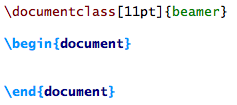
\includegraphics[scale=.5]{CODE1}
	\centering
\end{figure}

As there is nothing to compile, let's now turn to add information and material to our presentation. To do so, let's look at slides, or ``frames." \\

To add information into a single slide, we simply start a frame environment, type whatever we want, and then end that environment. This gives us a single slide. Then, we repeat for however many frames we need for our presentation (\textit{Note}: there are many ways to build and design slides, which we will get into in a bit). \\

So let's update our code with a single, simple frame,

\begin{figure}[!h]
	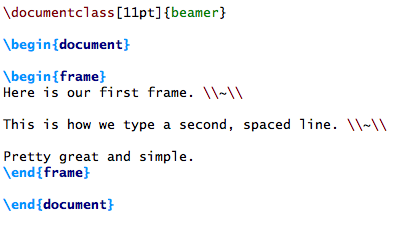
\includegraphics[scale=.5]{CODE2}
	\centering
\end{figure}

And this gives us a single slide with the information we included,

\begin{figure}[!h]
	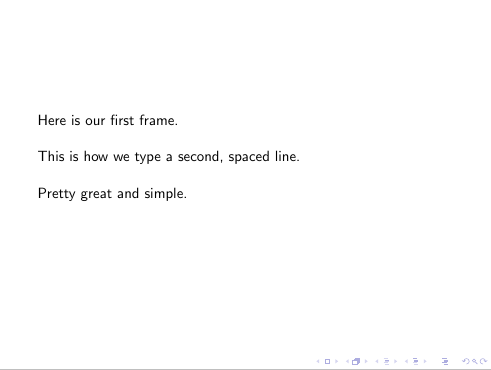
\includegraphics[scale=.5]{OUT2}
	\centering
\end{figure}

\newpage

Now, let's say we wanted to add a title slide. To do so, we need to add the identifying information \textit{prior} to starting the document (i.e., in our preamble). Then, \textit{after} we begin the document environment, we create a new frame that tells \LaTeX\ to make the information in the preamble the title for the whole presentation. To do so, let's type the following,

\begin{figure}[!h]
	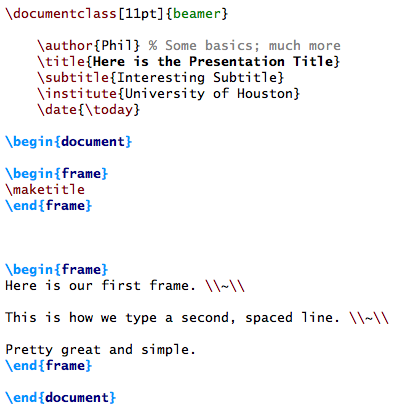
\includegraphics[scale=.5]{CODE3}
	\centering
\end{figure}

This gives us our two frames: title and the original frame...

\begin{figure}[!h]
	
\includegraphics[scale=.6]{OUT3}
	\centering
\end{figure}

\newpage

\subsection{Building a Single Frame}

\forceindent Now that we have a title and basic frame, let's create multiple frames based on a \textit{single} frame. We need to think of it this way, because we often add information a bullet at a time when presenting. Though you could build multiple frames manually (.e.g, a new frame environment for each new bullet), this can be a giant waste of time. Therefore, we will need to update twe things in our original presentation: a new frame environment within braces, and then the ``pause" command after each line, denoting a new frame after that line. Let's type the following code to get started,

\begin{figure}[!h]
	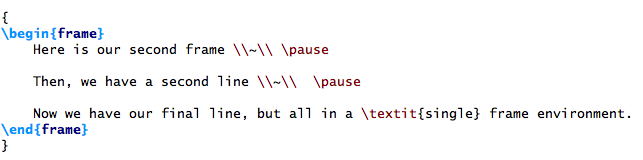
\includegraphics[scale=.6]{CODE4}
	\centering
\end{figure}

Though the output is too large to place in this document, the output should be three separate slides, each adding the successive item, as you coded using the ``pause" command. 

\subsection{Adding Frame Titles}

\forceindent To this point, we have only made simple, blank frames with information. Let's add a title to the frame to see the automatic formatting by \LaTeX. Simply include the command, ``frametitle" along with the specific title to add it to the frame. Start with,

\begin{figure}[!h]
	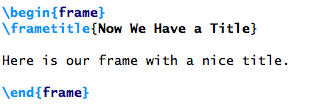
\includegraphics[scale=.6]{CODE5}
	\centering
\end{figure}

And this gives us, 

\begin{figure}[!h]
	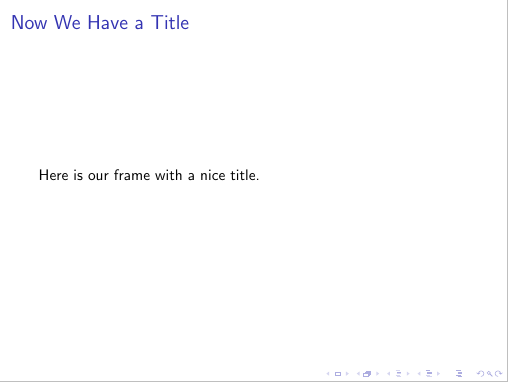
\includegraphics[scale=.5]{OUT5}
	\centering
\end{figure}

\subsection{Multiple Columns}

\forceindent We are starting to get better presentations. Let's add to this by splitting a frame into multiple columns. To do so, we will work within the ``columns" environment within our frame environment. Within this environment, we will specify the amount of columns we want by telling \LaTeX\ the amount to split the frame by (e.g., for two columns, we split it by $.5$; for three columns we split the frame by $.33$, etc.).\footnote{You could also vary the size of columns to make one small and the other large for example, as long as it adds up to 1. Try out options and different columns on your own.} Let's type the following to see how this works starting with two columns, three columns the same length, and then three columns different lengths,

\begin{figure}[!h]
	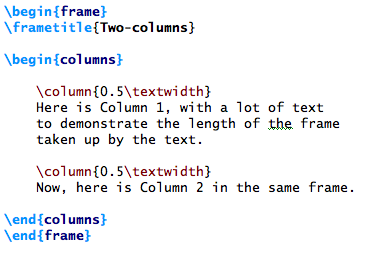
\includegraphics[scale=.6]{CODE6}
	\centering
\end{figure}

And this gives us a two-column frame as we expect, 

\begin{figure}[!h]
	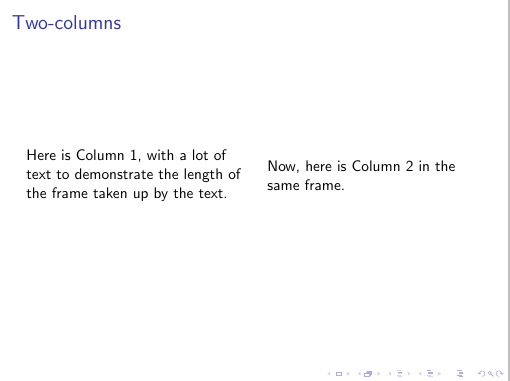
\includegraphics[scale=.5]{OUT6}
	\centering
\end{figure}

Next, for three same-length columns type:

\begin{figure}[!h]
	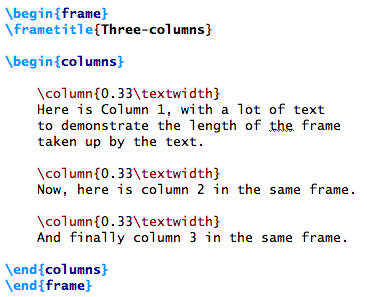
\includegraphics[scale=.6]{CODE7}
	\centering
\end{figure}

And this gives us a three-column frame, 

\begin{figure}[!h]
	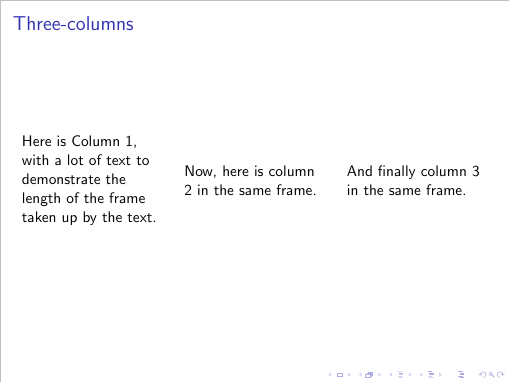
\includegraphics[scale=.5]{OUT7}
	\centering
\end{figure}

\newpage

And finally, for three columns, but of different lengths, type:

\begin{figure}[!h]
	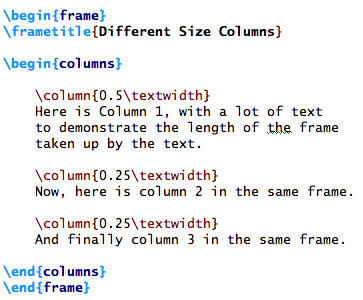
\includegraphics[scale=.6]{CODE8}
	\centering
\end{figure}

And this gives us a three-columns frame with different lengths, 

\begin{figure}[!h]
	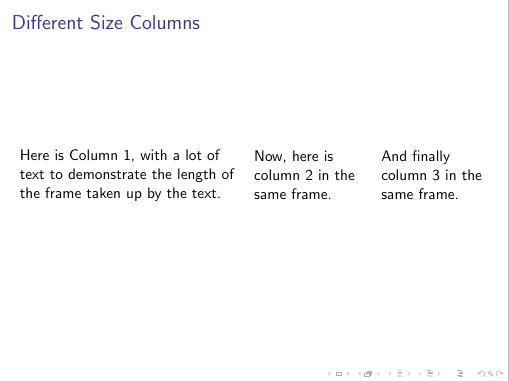
\includegraphics[scale=.5]{OUT8}
	\centering
\end{figure}

\subsection{Adding Figures, Tables, and Equations}

\forceindent Finally, to add Figures, Tables, and Equations in Beamer, you do this the same as you would in a document. This is a great feature of doing all work in \LaTeX\, whereby you can easily move stuff from a paper to a presentation and vice versa, without changing or updating formatting (for the most part). Thus, given that we have already done all of these things, but for articles, we are going to do a quick overview of each showing their applicability in Beamer. \\

Let's start with Figures. Remember to include the ``graphicx" package in your preamble, as well as setting your graphics path to where ever your image is stored to tell \LaTeX\ where to pull it. Thus, remember to save your image (a PNG if possible) in that folder, with a name including no spaces or punctuation). Start with the following,

\begin{figure}[!h]
	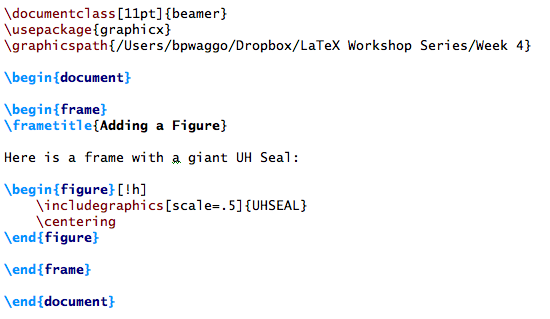
\includegraphics[scale=.6]{CODE9}
	\centering
\end{figure}

Now we have our slide with a giant UH seal included (remember you can resize the image using the ``scale" subcommand in brackets):

\begin{figure}[!h]
	
\includegraphics[scale=.5]{OUT9}
	\centering
\end{figure}

Next, let's add a table to our frame. To do so, remember we need the tabular environment exactly as before, only this time we include it within the frame environment. Start with the following,

\begin{figure}[!h]
	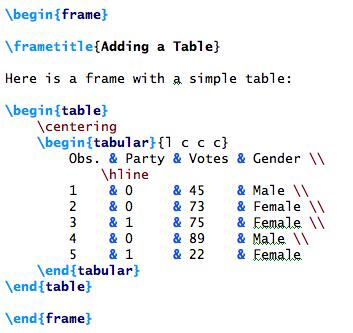
\includegraphics[scale=.6]{CODE10}
	\centering
\end{figure}

And here is our frame with a simple table,

\begin{figure}[!h]
	
\includegraphics[scale=.5]{OUT10}
	\centering
\end{figure}

Finally, let's see the inclusion of an equation in a frame, using the ``equation" environment. Start with,

\begin{figure}[!h]
	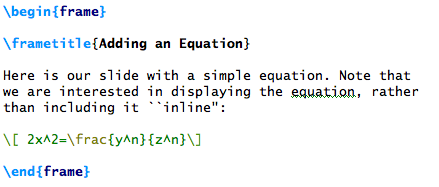
\includegraphics[scale=.6]{CODE11}
	\centering
\end{figure}

And here is our frame with a displayed equation, rather than ``inline,"

\begin{figure}[!h]
	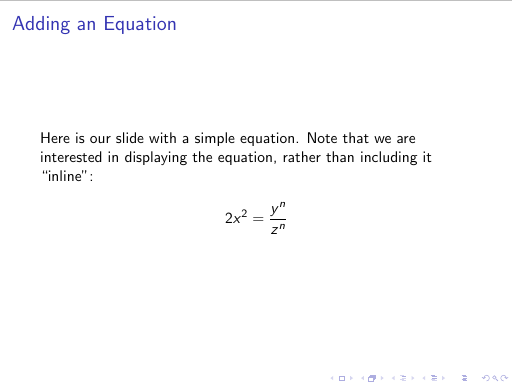
\includegraphics[scale=.5]{OUT11}
	\centering
\end{figure}

\end{document}
